\documentclass[12pt]{book}
\usepackage{multicol}
\usepackage{esvect}
\usepackage{amsmath}
\usepackage{amsthm}
\usepackage{graphicx}
\usepackage{color}
\usepackage[utf8]{inputenc}
\usepackage{framed,enumitem} 
\usepackage{pdfpages} 
\usepackage[english]{babel}
\usepackage[a4paper, total={6in, 9in}]{geometry}
%\newenvironment{proof}{\paragraph{Proof:}}{\hfill$\square$}
\usepackage{mathrsfs}
\usepackage{commath}
\usepackage{empheq,mathtools}
\usepackage[backend=biber, style=authortitle]{biblatex}
\addbibresource{References/references.bib}
\usepackage{mdframed}
\usepackage{multicol}
\usepackage{enumitem}
%\usepackage{unicode-math}
\usepackage[makeroom]{cancel}
\usepackage{import}
\usepackage{xifthen}
\usepackage{transparent}
\usepackage{amssymb}
\usepackage{tabularx}
\usepackage[bookmarks]{hyperref}
\newcommand{\incfig}[1]{%
    \def\svgwidth{\columnwidth}
    \import{./figures/}{#1.pdf_tex}
}
\pdfsuppresswarningpagegroup=1


\setcounter{tocdepth}{2}
\setcounter{secnumdepth}{2}

\newtheorem{theo}{Theorem}[section] % reset theorem numbering for each chapter
\newtheorem{defn}[theo]{Definition} % definition numbers are dependent on theorem numbers
\newtheorem{exmp}[theo]{Example} % same for example numbers
\newtheorem{cor}[theo]{Corollary} % same for corollary numbers
\newtheorem{prop}[theo]{Proposition} % same 
\newtheorem{lem}[theo]{Lemma} % same 

%make ftheo be framed theorems
\newenvironment{ftheo}
  {\begin{mdframed}\begin{theo}}
  {\end{theo}\end{mdframed}}
\newcommand{\qed}{\rule{2mm}{2mm}}

\makeatletter
\renewcommand*\env@matrix[1][*\c@MaxMatrixCols c]{%
  \hskip -\arraycolsep
  \let\@ifnextchar\new@ifnextchar
  \array{#1}}
\makeatother


\title{Geometry}
\author{Joel Andrepont, Lecturer : Boris Thibert}
\date{Fall 2019}
\begin{document}
\maketitle
\tableofcontents
\chapter{Introduction}
\section{Needs of CAGD}
\label{sec:Needs of CAGD}
\begin{itemize}
  \item Design curves or surfaces
  \item Bezier curves : $ \\ $Introduced in the 70s
      \begin{itemize}
          \item Pierre Bezier (Renault)
          \item De Casteljau (Citreon)
      \end{itemize}
  \item We want polynomials that are smooth without sharp corners. Want local movement so
      we can change aspects of the curve rather than the entire curve. 
  \item We stitch together polynomials in order to avoid Runge phenomenon. 
\end{itemize}

\section{Lagrange Interpolation}
\label{sec:Lagrange Interpolation}
\begin{defn}[Problem]
$ \\ $    We have $ y_0, \cdots, y_n \in  \mathbb{R}^d $ and parameters $ t_0, \cdots,
    t_n \in \mathbb{R}$.
    We want to find a function 
    \[
        f : [t_0, \cdots, t_n] \to \mathbb{R}^d, \mathscr{ C }^d  \text{ such that } f(t_i) = y_i \qquad
        0 \leq i \leq n
    \]
    \label{def:Problem}
\end{defn}
\newpage 
\subsection{Lagrange polynomial}
\label{subsec:Lagrange polynomial}
We find a solution which is a polynomial. 
\begin{ftheo}[Lagrange Polynomial] $ \\ $
    Let $ y_0, \cdots, y_n  \in \mathbb{R}^d$ with $ a = t_0 < \cdots < t_n = b $ real
    numbers. $ \\ $
    There exists a unique polynomial $ L_n $ that satisfies 
    \[
        L_n(t_i) = y_i \qquad \text{ deg}\left( L_n\right)  \leq n
    \]
    see drawing for cases of degree $ < n $. For instance, in the case where all the
    points fall on a straight line.
    \label{th:Lagrange Polynomial}
\end{ftheo}
The polynomial function $ L_n $ is given by 
\[
    L_n(t) = \sum_{i=0}^{n} y_i P_i(t)  
\]
where 
\[
    P_i(t) = \frac{ \prod_{j\neq i} \left( t - t_j\right)  }{ \prod_{j\neq i} \left( t_i -
    t_j \right)  } \qquad \begin{cases}
        P_i(t_j) &= 0 \text{ if } j \neq i \\
                 &=1 \text{ if } j = i
    \end{cases}
\]

\begin{proof} $ \\ $
    We denote $ E : $ the space of polynomial functions of degree $ \leq n  $.
    $ E \subset \mathbb{R}^{n+1} $.
    Consider the map 
    \begin{align*}
        \varphi : &E \to \mathbb{R}^{n+1} \\ 
                  &P \to \left( P(t_0) , \cdots , P(t_n) \right) 
    \end{align*}
    is a linear map, to show this consider $ P,Q $ and $ \alpha \in \mathbb{R}$. 
    \begin{align*}
        (\alpha P + Q)  &= 
        \begin{pmatrix*}
           \alpha P\left( t_0\right) + Q\left( t_0\right)   \\
             \vdots \\
             \alpha P\left( t_n\right) + Q\left( t_n\right) 
        \end{pmatrix*}
         =
        \left(\begin{pmatrix*}
             \alpha P\left( t_0\right)  \\
             \vdots \\
             \alpha P\left( t_n\right) 
        \end{pmatrix*}
        + \begin{pmatrix*}[r]
             Q\left( t_0\right)  \\
             \vdots \\
             Q\left( t_n\right) 
        \end{pmatrix*} \right) 
        \\ 
                        &= \alpha \begin{pmatrix*}
             P\left( t_0\right) \\
              \vdots \\
              P\left( t_n\right) 
         \end{pmatrix*}
         + \begin{pmatrix*}
             Q\left( t_0\right)  \\
             \vdots \\
             Q\left( t_n\right) 
         \end{pmatrix*} \\
                        &= \alpha \varphi \left( P\right) + \varphi \left( Q\right)  
    \end{align*} 
    For uniqueness we need to show that $ \varphi $ is bijective. 
    We will prove that $ \varphi $ and indeed any linear map is injective if the null
    space of the map is the set $ \set{0} $. $ \\ $. 
    \begin{lem}[Linear maps take 0 to 0] $ \\ $
        Suppose $ T $ is a linear map that takes $ V\to W $. Then $ T(0) = 0 $. 
        \begin{proof}
            Since T is linear, we have : 
            \[
                T(0) = T(0 + 0) = T(0) + T(0) 
            \]
            which is only true when $ T(0) = 0 $
        \end{proof} 
        \label{lem:Linear maps take 0 to 0}
    \end{lem} 
    \begin{lem}[Injectivity is equivalent to null space equals \{0\}]
        $ \\ $Let $ T \in \left( V,W\right)  $. Then T is injective if and only if null $ T =
        \set{0} $
        \label{lem:Injectivity is equivalent to null space equals 0}
    \end{lem}
    \begin{proof}
        First, suppose that $ T $ is injective. We want to prove that null $ T = \set{0}
        $. By \ref{lem:Linear maps take 0 to 0} we know that $ \set{0} \subset  $ null $ T
        $. To prove the inclusion in the other direction suppose that $ v \in N\left(
        T\right)  $(null of T). Then 
        \[
        T(v ) = 0 = T(0) 
        \]
        Since $ T $ is injective, this implies that $ v = 0 $. Therefore we can conclude
        that $ N\left( T\right) = \set{0} $ as desired. 
        To prove the other direction we begin with $ N\left( T\right) = \set{0}  $ and
        want to show that $ T $ is injective. Suppose $ u,v \in V $. and $ Tu = Tv $.
        Then 
        \[
            0 = Tu - Tv = T(u-v) 
        \]
        thus $ u-v  $ is in $ N\left( T\right)  $ which is $ \set{0}  $. Hence, $ u-v = 0
        $ which implies that $ u = v  $. Hence $ T $ is injective. 
    \end{proof}
    The last theorem we need is the Fundamental Theorem for Linear Maps. 
    \begin{ftheo}[Fundamental Theorem of Linear Maps]
        Suppose $ V $ is finite-dimensional and $ T \in \mathcal{ L } \left( V,W\right)
        $. Then the range $ T $ is finite-dimensional and 
        \[
        \text{dim } V = \text{ dim } \mathcal{ N } \left( T\right) + \dim \mathcal{ R }
        \left( T\right)  
        \] where $ \mathcal{ R  } \left( T\right)  $ is the range. 
        \label{th:Fundamental Theorem of Linear Maps}
    \end{ftheo}
    We supply the definition for surjective and injective functions in order to begin the
    proof. 
    \begin{defn}[Injective]
        A function $ T : V \to W $ is called injective if $ Tu = Tv  $ implies $ u = v.
        $
        \label{def:Injective}
    \end{defn}
    \begin{defn}[Surjective]
        A function $ T : V \to W $ is called surjective if its range equals $ W $.
        \label{def:Surjective}
    \end{defn}
    We can finally now prove \ref{th:Lagrange Polynomial}. We have that $ \varphi  $ is a
    linear map. The kernel/nullspace of $ \varphi  $ is given by. 
    \[
        \mathcal{ N  } \left( \varphi \right) = \set{ P \in E : \varphi\left( P\right) = 0 } 
    \]
    Thus, 
    \[
    \exists  P \in E, \qquad \varphi = \begin{pmatrix*}
         0 \\
         \vdots \\
         0
    \end{pmatrix*}
    \]
    Then $ P\left( t_i\right) = 0 \ \forall i \in \set{ 0,\cdots, n}  $ where P is of
    degree $ \leq n $. Now, we can write our polynomial as 
    \[
       P =  a_1 + a_2x + a_3x^2 + \cdots + a_nx^{n-1}
    \]
    Where $ P\left( t_0\right) = a_1 + a_2t_0 + \cdots + a_nt_0 = 0 $. We can proceed by
    induction using differentiation to show that 
    \begin{align*}
        P' &= a_2 + 2a_3(t_1) + \cdots + \left( n-1\right) a_nt_2^{ n-2 } \implies a_2 = 0  
    \end{align*}
    and so on. Giving us that the kernel of $ \varphi $ is $ \set{ 0 }  $. Using
    \ref{th:Fundamental Theorem of Linear Maps} we have 
    \begin{align*}
        \text{dim} E &= \text{dim } \mathcal{ N } \left( \varphi \right) + \text{ dim }
        \mathcal{ R  } \left( \varphi\right) \\ 
                     &= 0 + \text{ dim } \mathcal{ R  } \left( \varphi\right)   
    \end{align*} 
    By \ref{lem:Injectivity is equivalent to null space equals 0} and \ref{def:Surjective}
    we have that $ \varphi  $ is bijective and uniqueness of the polynomial used to
    represent each set of real numbers $ \left( y_0, \cdots, y_n \right) \in \mathbb{R}^d $
\end{proof}

\subsection{Runge Phenomenon}
\label{subsec:Runge Phenomenon}
Consider the function
\[
    f(x) = \frac{ 1 }{ 1 + 25x^2 } \qquad \text{ on } [-1,1]
\]
where $ t_0, \cdots, t_n $ are uniformly distributed on the interval and $ y_i = f(t_i) $

\subsection{Approximation Result}
\label{subsec:Approximation Result}
\begin{ftheo}[]
    $ \\ $
    Let $ f : [a,b] \to \mathbb{R} $ of class $ \mathscr{ C }^{n+1}  $
    and $ L_n  $ the lagrance polynomial associated to $ f $ and the nodes $ a = t_0 < \cdots
    < t_n = b$ $ \\ $
    Then 
    \[
        \| f - L_n \|^{ }_{ \infty} \leq \frac{ 1 }{ \left( n+1\right) ! } \| q_{n+1} \|^{
        }_{ \infty } \| f _{  }^{ (n+1) }  \|^{ }_{ \infty} 
    \]
    where $ q _{ n+1 }^{  } (t) = \prod _{ i=0 }^{ n  } \left( t - t_i\right)  $
    \label{th:}
\end{ftheo}
$ \| q _{ n+1 }^{  }  \|^{ }_{ \infty}  $ is dependent on the interval. Also, $ \| f _{
}^{ (n+1) }  \|^{ }_{ \infty}  $ is also unknown. These two can go towards infinity
depending on the function and the interval.

\begin{proof}
    We introduce the error function 
    \[
    g \coloneqq f - L_n 
\] and we fix $ t \in [a,b] \setminus \set{ t_i }    $ and we also define 
\[
    k(u) \coloneqq g(u) - \frac{ q _{ n+1 }^{  } (u)g(t) }{ q _{ n+1 }^{  } (t) } 
\]
Note that $ \forall i $ we have 
\begin{align*}
    g(t_i)  &= f(t_i) - L_n\left( t_i\right)  \\ 
            &= f(t_i) - \sum_{k=0}^{n} y_k P_k(t_i) \\
            &P_k\left( t_i\right) = 0 \ \forall k \neq i \text{ and } = 1 \text{ if } k=i \\
     g\left( t_i\right)  &= f\left( t_i\right) - y_k\left( 1\right) \\
                       0  &= y_k - y_k \\ 
\end{align*}
Furthermore, 
\subsection{Need to check this}
\label{subsec:Need to check this}


\begin{align*}
    k(t_i) &= g(t_i) - \frac{ q _{ n+1 }^{  } (t_i) g(t) }{ q _{ n+1 }^{  } (t) } \\
     &= 0 -  \frac{ q _{ n+1 }^{  } (t_i) \left( 0\right)  }{ q _{ n+1 }^{  } (t) } = 0\\ 
\end{align*}

We now consider when $ t \neq t_i $. The function $ g $ has n+2 distinct real roots, each
at $ t = x $ and $ t = x_i $ for $ i \in \set{ 0,\cdots, n }  $. 
We also have $ k(t) = 0$ then $ k $ vanishes
at $ \left( n+2\right)  $ points then by Rolle's theorem (Mean Value Theorem) $ k' $ vanishes at (n+1)
$ \\ $
$ \implies  $ $ k _{  }^{ (n+1) }  $ vanishes at one point denoted by $ \xi  $. 
$ \\ $
\[
    k _{  }^{ n+1 } (\xi) = 0
\]
A calculation gives 
\[
    0 = k _{  }^{ (n+1) }(\xi) = g _{  }^{ (n+1) } (\xi) - q _{ n+1 }^{ (n+1) } (\xi) \frac{
    g(t) }{ q _{ n+1 }^{  } (t) } 
\]
However, 
Since $ L_n  $ has dimension $ \leq n  $ then $ g _{  }^{ (n+1) } = f  _{  }^{ (n+1)  } $ 
and $ q _{ n+1 }^{  } (\xi) = \left(n+1\right) ! $ since it is simply the $ (n+1) $
derivative of a polynomial with leading term $ t _{  }^{ (n+1) }  $.  
Then 
\[
    f _{  }^{ (n+1) } \left( \xi\right) = \left( n+1\right) ! \frac{ g(t) }{ q _{ n+1 }^{
    } (t)  } 
\]
Then 
\[
    \left | g(t) \right | = \frac{ 1 }{ \left( n+1\right) ! } \| q _{ n+1 }^{  } (t)  \|^{
    }_{ } \left | f _{  }^{ (n+1)  } (\xi) \right | \leq \frac{ 1 }{ \left( n+1\right) ! }
    \| q _{ n+1 }^{ (t)  }  \|^{ }_{ \infty } \| f _{  }^{ (n+1) }  \|^{ }_{ \infty } 
\]
\end{proof}


\section{Exercise 1 : Lagrange interpolation}
\label{sec:Exercise 1 : Lagrange interpolation}
We first recall the Lagrange Polynomial         
\begin{defn}[Lagrange Polynomial]
    Let $ f L [a,b] \to \mathbb{R} $ be a function and $ a\leq x_0 \leq \cdots \leq x_n
    \leq b $ in [a,b]. The Lagrange polynomial is given by 
    \[
        L_n(x) = \sum_{i=0}^{n} y_iP_i(x)\text{, where } P_i(x) = \frac{
        \prod_{j\neq i}\left( x-x_j\right)  }{ \prod_{j\neq i} \left( x_i - x_j\right)  } 
    \]
    \label{def:Lagrange Polynomial}
\end{defn}

The goal of this exercise is to use another formulation for the Lagrange Polynomial, whose
calculation is less costly. 
\begin{enumerate}[]
    \item Using the above formulation, estimate the number of operations to evaluate
        $ L_n(x) $. 
    \item Show that the $ n+1 $ functions 
        \[
        x\to1, \text{ and } x\to\left( x-x_0\right) \cdots\left( x-x_k\right) , \ 0\leq k
        \leq n-1 
    \] form a basis for the set of polynomial functions on $ [a,b] $ of degree $ \leq  n$. 
\item We now denote by $ L_k  $ the lagrange polynomial of degree $ \leq n $ that
    satisfies $ L_k(x_i) = f(x_i) $ for $ 0\leq i \leq k $. We also denote by $ f[x_0,
    \cdots, x_k ] $ the dominant coefficient. Show by induction that 
    \[
        L_n(x) = f(x_0) + \sum_{k=1}^{n} f[x_0, \cdots, x_k] \left( x-x_0\right) \cdots 
        \left( x-x_{k-1}\right) 
    \]
\item Show that for every $ k\geq 1 $
    \[
        f[x_0, x_1, \cdots, x_k] = \frac{ f[x_1, \cdots, x_k] - f[x_0, \cdots, x_{k-1}  }{
        x_k - x_0 } \text{ and } f[x_i] = f(x_i)
    \] 
\end{enumerate} 
\subsection{Solutions }
\subsubsection{1)}
We have n+1 points, thus, for 
\[
    \sum_{i=0}^{n} y_i P_i(x) 
\]
$ P_i(x)  $ gives us n multiplications and n divisions, which is $ \mathcal{ O  } (n)  $.
Since we do this n times we have $ \mathcal{ O  }(n^2)$. 

\subsubsection{2)}
\begin{proof}
Let $ \psi_i  $ be functions such that 
\begin{align*}
    \psi_{-1} &\to 1  \\ 
    \psi_0 &\to (x-x_0)  \\ 
    \psi_1 &\to (x-x_0)(x-x_1)  \\ 
           &\vdots \\
    \psi_n &\to (x-x_0)(x-x_1)\cdots\left( x-x_{n-1}\right)   \\ 
\end{align*}
it is sufficient to show that $ \left( \psi_{-1}, \cdots, \psi_{n-1} \right)  $ is
linearly independent.
To do this, consider 
\[
    P(x) = C_0\psi_{-1} + C_1\psi_{0} + \cdots + C_n\psi_{n-1} = 0
\]

if $ x = x_0 $ then 
\[
    P(x_0) = C_0 + 0 = 0 \iff C_0 = 0
\]
Likewise, if $ x = x_1 $
\[
    P(x_1) = 0 + C_1\psi_0  + 0 = 0 \iff C_1 = 0
\]
we can continue this for all $ x_i$ where $ i \in \set{ -1, \cdots, n-2 }  $. Finally
giving us 
\[
    P(x_{n-2}) = 0 + 0 + \cdots + 0 + C_n\psi_{n-1} = 0 \iff C_n = 0
\] 
\end{proof}

\subsubsection{3)}
For $ k=0 $ we simply have 
\[
    L_0(x_0) = f(x_0)  
\]
for $ k=1 $ we have 
\[
    L_1(x_1) = f(x_0) + f[x_0, x_1](x-x_0)  
\]
for $ k + 1 $ we have 
\begin{align*}
    L_{k+1} (x) &= L_k(x) + f[x_0, \cdots, x_{k-1} ] \left( x-x_0\right) \cdots\left(
    x-x_k\right) \\
        \underbrace{ L_{k+1}(x) - L_k(x)}_{\text{polynomial of degree } \leq k+1 } &= f[x_0, \cdots, x_{k-1} ] \left( x-x_0\right) \cdots\left( x-x_k\right)
\end{align*}
this polynomial vanishes at $ x_0, \cdots, x_k $ or $ k+1  $ values. Then $ \alpha  $ is
the dominant coefficient given by $ L_k(x) + f[x_0, \cdots, x_{k-1} ] $.  

\section{Interpolation with Splines}
\label{sec:Interpolation with Splines}

The goal is to have piecewise polynomial curve with smooth gluings. 

\begin{figure}[ht]
    \centering
    \incfig{piecewisepoly}
    \caption{piecewise polynomial interpolation}
    \label{fig:piecewisepoly}
\end{figure}


\begin{ftheo}[Cubic B-spline]
    Let $ y_0, \cdots, y_n \in \mathbb{R}^{n+1} $ with $ a=t_0 < \cdots < t_n = b $ and $
    \alpha, \beta \in \mathbb{R}$. There exists a unique 
    \[
        S : [a,b] \to \mathbb{R} \qquad \text{ such that } 
    \]
    \begin{enumerate}[label={(\roman*)}]
        \item $ S _{ [t_i, t_{i+1} ] }^{  }  $ is polynomial of degree $ \leq 3 $. 
        \item $ S $ is of class $ \mathscr{ C } ^2 $
        \item $ S(t_i) = y_i $
        \item $ S'(a) = \alpha  $ and $ S'(b) = \beta  $
    \end{enumerate}
    \label{th:cubicBspline}
\end{ftheo}

Sketch of proof
\begin{proof} $ \\ $
    \begin{enumerate}
        \item We denote $ \mathscr{ P }  $ the space of functions $ f : [a,b] \to \mathbb{R}$ of 
            class $ \mathscr{ C } ^2 $ which are polynomials of degree $ \leq 3 $ on each
            $ [t_i, t_{i+1}] $.
            \begin{itemize}
              \item $ \mathscr{ P }  $ is a vectorial space
              \item dim $ \left( \mathscr{ P } \right)  $ is $ 4*n $ where n is the number
                  of intervals and 4 is given by the number of parameters to find each
                  point. 
              \item We have 3 conditions for each point if we want to uphold $ \mathscr{ C
                  } ^2 $ continuity. 
                  \begin{itemize}
                      \item $ P_i(t_i) = P_{i+1}(t_i) $ 
                      \item $ P_i'(t_i) = P'_{i+1}(t_i) $ 
                      \item $ P_i''(t_i) = P''_{i+1}(t_i) $ 
                  \end{itemize}
            \end{itemize} 
        \item A solution $ S \in \mathscr{ P }  $ of the theorem satisfies 
            \begin{enumerate}
                \item $ S'\left( a\right) = \alpha  $
                \item $ S'\left( b\right) = \beta  $
                \item $ S\left( t_i\right) = y_i, \ \forall i \in \set{ 0, \cdots, n }  $
            \end{enumerate}
            Each line is a linear system in the set of paramters i.e. $ S'(a) = \alpha  $
            and we know that 
            $ S(x) = a_0 + a_1x + a_2x^2 + a_3x^3  $ on $ [t_0, t_1]  $ and 
            $ S'(\alpha) = a_1 + 2x^2 + 3a_3x^2 = \alpha  $ linear in $ \left( a_0, a_1,
            a_2, a_3\right)  $. These equations are independent (ADMITTED). Thus, there exists
            a unique solution. 
    \end{enumerate}
\end{proof}

\begin{figure}[ht]
    \centering
    \incfig{cubicbspline}
    \caption{cubicBSpline}
    \label{fig:cubicbspline}
\end{figure}

\subsection{Minimization Result}
\label{subsec:Minimization Result}
\begin{ftheo}[]
    Let $ y_0, \cdots, y_n \in \mathbb{R}^{n+1}  $ $, a = t_0, \cdots, t_n = b $. $ S  $
    the spline associated to this interval.  
    Then, 
    \[
    S = argmin \int\limits_{a}^{b} f''(t) ^2 \ dt \qquad f \in E 
    \]
    Where $ E = \set{ f:[a,b] \to \mathbb{R} \text{ of class } \mathscr{ C } ^2, f'(a) =
    \alpha, f'(b) = \beta, f(t_i) = y_i }  $ This is to say that the spline is the
    solution to this problem with the least curvature or minimal energy. 
    \label{th:minResult}
\end{ftheo}
\begin{proof}
    Let $ f\in E $, $ e = f - S $ the error. 
    \begin{enumerate}
        \item First, we show that for every function $ h : [a,b]  $ piecewise linear
            continuous on each $ [t_i, t_{i+1} ]  $ 
\begin{figure}[ht]
    \centering
    \incfig{hpwlin}
    \caption{h(t)} 
    \label{fig:hpwlin}
\end{figure}       
$ \\ $
            One has : 
            \[
                \int\limits_{a}^{b} e''(x)h(x) = 0
            \]
            Indeed, 
            \begin{align*}
                \int\limits_{a}^{b} e''(x)h(x) =& \sum_{i=0}^{n-1}
                \int\limits_{t_i}^{t_{i+1}} e''(x)h(x) \ dx \\
                                                &= \sum_{i=0}^{n-1} \left( \left[e'(x)h(x)
                                                \right] _{ t_i }^{ t_{i+1}  } - 
                                                \int\limits_{t_i}^{t_{i+1} } e'(x)h'(x) \
                                            dx \right) \\
            \end{align*}
            for the left hand term we have 
            \[
                e'(b)h(b) - e'(a)h(a) = 0 
            \] since 
            \[
                e'(b) = f'(b) - S'(b) = 0 \text{ and } e'(a) = f'(a) - S'(a) = 0 
            \]
            For the right hand term 
            \[
                h'(x) = \lambda_i \text{ on } [t_i, t_{i+1} ]  
            \]
            Then 
            \begin{align*}
                \sum_{i=0}^{n-1} \int\limits_{t_i}^{t_{i+1} } e'(x) \lambda_i \ dx 
                = -\sum_{i=0}^{n-1} \lambda_i \left( e\left(
                t_{i+1}) - e(t_i) \right) \right)  \ dx 
            \end{align*}
            indeed 
            \[
                e(t_i) = f(t_i) - S(t_i) = y_i - y_i = 0
            \]
        \item 
            \begin{align*}
                \int\limits_{a}^{b} \left(f''(x)\right)^2 \ dx &= \int\limits_{a}^{b} \left( e''(x) +
                    S''(x)
                \right) ^2 \ dx \\
                                                               & = \int\limits_{a}^{b}
                                                               \left(e''(x)\right)^2 \ dx 
                                                               + \int\limits_{a}^{b}
                                                               \left(S''(x)\right)^2 \ dx + 2
                                                  \int\limits_{a}^{b} e''(x)S''(x) \ dx
            \end{align*} 
            S is piecewise poly of degree $ \leq 3 $. 
            Then $ h = S'' $ piecewise linear then 
            \[
            \int\limits_{a}^{b} e''h \ dx= 0
        \] from step (1). 
        Then 
        \[
            \int\limits_{a}^{b} \left(f''(x)\right)^2 \ dx = \int\limits_{a}^{b}
            \left(e''(x)\right)^2\ dx +
            \int\limits_{a}^{b} \left(S''(x)\right)^2 \ dx
        \]
        Then 
        \[
            \int\limits_{a}^{b} \left(f''(x)\right)^2 \ dx \geq \int\limits_{a}^{b}
            \left(S''(x)\right)^2 \ dx 
    \] (S is a minimizer, by assumption). 
    We have equality if and only if 
    \[
        \int\limits_{a}^{b} \left(e''(x)\right)^2 \ dx = 0 \iff e''(x) = 0 \text{ because } e'' \text{ is continuous }  
    \] 
    Using $ e(t_i) = 0 $ $ e'(a) = e'(b) = ? \then e \equiv 0 $.  
    \end{enumerate}
\end{proof}
If $ f'' \equiv 0 \implies f' = a \implies f(x) = Ax + B$ we don't want zero, but we do
want minimization of curvature. 



\subsection{Approximation Result}
\label{subsec:Approximation Result}
\begin{ftheo}[]
    Let $ f:[a,b] \to \mathbb{R} \in \mathscr{ C } ^2 $. $ S  $ the spline associated to $
    a = t_0 < \dots < t_n = b$. and $ y_i = f(t_i)  $. 
    Then, 
    \[
        \| f - S \|^{ }_{ \infty } \leq \frac{ h^{3/2}  }{ 2 } \| f \|^{ }_{ 2} 
    \]
    with $ h = \max \left | t_i - t_{i+1}  \right |  $
    \[
        \| f' - S' \|^{ }_{ \infty } \leq h^{1/2} \| f'' \|^{ }_{ 2} 
    \]
    \label{th:}
\end{ftheo}
\begin{proof}
    We put $ e = f - S $. 
    \[
    \| e'' \|^{ 2}_{ 2} = \int\limits_{a}^{b} e''^2 = \int\limits_{a}^{b} f''^2 -
    \int\limits_{a}^{b} S''^2 
    \]
    \begin{equation}
        \leq \int\limits_{a}^{b} f''^2 = \| f'' \|^{ 2}_{ 2} \text{ (*) } 
        \label{eq:fNorm}
    \end{equation}
    $ \forall i,\ e(t_i) = 0  $ By Rolle's theorem, this implies 
    $ \forall i, \ \exists \xi i \in [t_i, t_{i+1} ]  $ s.t. $ e'(\xi_i) = 0  $
    Then 
    \[
        \forall i \in [a,b] ,\ \exists t' \in [a,b] \text{ s.t. } e'(t') = 0 \text{ and }
        \left | t - t'  \right | \leq h
    \]
    Then 
    \begin{align*}
        \left | a'(t)  \right | &\leq \left | e'(t) - e'(t')  \right | \\
                                &\leq \left | \int\limits_{t}^{t'} e''(s) \ ds \right |  \\ 
                                &\leq \left | \int\limits_{t}^{t'} ds \right | ^{1/2} 
                                \left | \int\limits_{t}^{t'} e''(s)^2 ds \right | ^{1/2}
                                \text{ C.S. } \\ 
                                &\leq h^{1/2} \| e'' \|^{ }_{ 2}  \\ 
                                &\leq h^{1/2} \| f'' \|^{ }_{ 2} \text{ by (*)}  \\ 
    \end{align*}
    Second inequality : 
    $ \\ $
    Since $ e(t_i) = 0 \implies \forall t \in [a,b] \ \exists t''  $ s.t. 
    \[
    \left | t '-  t''  \right | < \frac{ h }{ 2 } \text{ and } e(t'') = 0
    \]
    \begin{align*}
        \left | e(t)  \right | &\leq \left | e(t) - e(t'')  \right | \\
         &\leq \left | \int\limits_{t}^{t''} e'(s) \ ds  \right | \\
         &\leq \left | t - t'' \right | 
         \| e' \|^{ }_{ \infty } \\ 
    \end{align*}
    The left side we have $ \leq \frac{ h }{ 2 }  $ and for the right side we have $
    h^{1/2} \| f'' \|^{ }_{ 2}  $ 
    Which gives : 
    \[
        \frac{ h^{3/2}  }{ 2 } \| f'' \|^{ }_{ 2} 
    \]
\end{proof}
\section{Exercise 2 : Hermite Interpolation }
\label{sec:Exercise 2 : Hermite Interpolation }
Let $ p  $ and $ q $ be two point of $ \mathbb{R}^d $ and $ \boldsymbol{u} , \boldsymbol{v}
\in \mathbb{R}^d  $ two vectors. The goal of this exercise is to find a polynomial curve $ \gamma :
[0,1] \to \mathbb{R}^d $ that interpolates the points and its derivatives, namely that
satisfies 
\[
    \gamma(0) = p \quad \gamma'(0) = \boldsymbol{u} \quad \gamma(1) = q \quad \gamma'(1) =
    \boldsymbol{v} 
\]
We first assume that $ d=1 $. The function $ \gamma : [0,1] \to \mathbb{R} $ is thus a
polynomial function, whose degree is denoted by $ k $. 
\begin{enumerate}
    \item What is the minimal degree $ k $ that we have to take if we want to expect a
        unique solution for any $ p, q, \boldsymbol{u} , \boldsymbol{v }  $? 
    \item Calculate the coefficients of such a polynomial function $ \gamma $ 
    \item Write $ \gamma $ under the form 
        \[
            \gamma(x) = ph_0(x) + qh_1(x) + \boldsymbol{u} h_2(x)+ \boldsymbol{v} h_3(x)
        \]
        where $ h_i $ are the polynomial functions to be determined. 
$ \\ $    We now suppose that $ d \geq 1 $. 
    \item Can we still write $ \gamma  $ under the form 
        \[
            \gamma(x) = ph_0(x) + qh_1(x) + \boldsymbol{u} h_2(x)+ \boldsymbol{v} h_3(x)
        \]
    \item Consider $ [a,b] $ with partition $ a = x_0 < \dots < x_n = b $ of $ [a,b] $
        with a set of points $ p_0, \cdots, p_n $ and set of vectors $ \boldsymbol{u} _0,
        \cdots, \boldsymbol{u_n} $
        Determine the curve $ \gamma : [a,b] \to \mathbb{R}^d $ which is polynomial of
        degree $ k $ on each interval $ [x_i, x_{i+1}]  $ and that satisfies 
        \[
            \gamma(x_i) = p_i \quad \text{ and } \quad \gamma'(x_i) = \boldsymbol{u} _i
        \]
\end{enumerate}
\subsection{Solutions}
\label{subsec:Solutions}
\subsubsection{1)}
We treat each of these conditions as a linear system. For the solution to be unique we
must solve a system with 4 conditions and 4 unknowns, therefore $ k =4 $. 

\subsubsection{2)}
We have 
\begin{align*}
    \gamma(0) &= p \\
    \gamma'(0) &= \boldsymbol{u}  \\ 
    \gamma(1) &= q \\ 
    \gamma'(1) &= \boldsymbol{v }  
\end{align*}
Consier that $ k = 4 $ we have 
\begin{align*}
    \begin{pmatrix}[cccc|c]
        a_0& 0& 0& 0& p \\
        0& a_1& 0& 0& \boldsymbol{u}  \\
        a_0& a_1& a_2& a_3&  q\\
        0& a_1& 2a_2& 3a_3&  \boldsymbol{v} \\
    \end{pmatrix}
     &\implies a_0 = p \text{ and } a_1 = \boldsymbol{u}  \\ 
\end{align*}
This gives us 
\[
p + \boldsymbol{u} + a_2 + a_3 &= q \implies a_2 + a_3 = q - p - \boldsymbol{u}  
\]
\[
\boldsymbol{v } = \boldsymbol{u} + 2\left( q - p - \boldsymbol{u} \right)  
+ a_3 \implies a_3 = \boldsymbol{u} + \boldsymbol{v } -2q + 2p
\]
Simple calculations show that 
\begin{align*}
    a_0 &= p \\ 
    a_1 &= \boldsymbol{u}  \\ 
    a_2 &= -3p + 3q - 2\boldsymbol{u} - \boldsymbol{v }  \\ 
    a_3 &=  2p - 2q + \boldsymbol{u} + \boldsymbol{v} \\ 
\end{align*}

\subsubsection{3)}
The equation can be written as 
\[
            \gamma(x) = ph_0(x) + qh_1(x) + \boldsymbol{u} h_2(x)+ \boldsymbol{v} h_3(x)
\]
where 
\begin{align*}
    h_0(x)  &= 1 -3x^2 + 2x^3 \\ 
    h_1(x) &= 3x^2 - 2x^3 \\ 
    h_2(x) &= x -2x^2 + x^3 \\ 
    h_3(x) &= -x^2 + x^3 \\ 
\end{align*}

\subsubsection{4)}
Yes, we simply denote 
\[
    \gamma_i(x) = p_ih_0(x) + q_ih_1(x) + \boldsymbol{u}_ih_2(x)+ \boldsymbol{v}_ih_3(x)
\]
we then have 

\[
    \gamma(x) = 
    \begin{pmatrix*}
        p_0 \\
        \vdots \\
        p_{n-1}
    \end{pmatrix*}h_0(x) + 
    \begin{pmatrix*}
        q_0 \\
        \vdots \\
        q_{n-1}
    \end{pmatrix*}h_1(x) + 
    \begin{pmatrix*}
        \boldsymbol{u} _0 \\
        \vdots \\
        \boldsymbol{u} _{n-1}
    \end{pmatrix*}h_2(x) + 
    \begin{pmatrix*}
        \boldsymbol{v}_0  \\
        \vdots \\
        \boldsymbol{v}_{n-1} 
    \end{pmatrix*}h_0(x) 
\]

\subsubsection{5)}
We first want to have $ t_i, t_{i+1}  $ to be $ [0,1] $
Thus, for $ t \in [t_i, t_{i+1}]  $ we have 
\[
    \frac{ t - t_i }{ t_{i+1} - t_i } 
\]
which then gives us 
\[
\gamma\left( \frac{ t - t_i }{ t_{i+1} - t_i }\right) 
\]
However, we see that the derivate of $ \gamma  $ gives 
\[
    \gamma'\left( \frac{ t - t_i }{ t_{i+1} - t_i }\right) = \frac{ 1  }{ 
    \left( t_{i+1} - t_i \right) } \gamma \left( \frac{ t - t_i }{ t_{i+1} - t_i } \right)  
\]
Thus, our equation now becomes 
\[
\gamma \left( \frac{ t - t_i }{ t_{i+1} - t_i }\right) = 
p_ih_0(x) + p_{i+1}h_1(x) + \left( t_{i+1} - t_i \right) \boldsymbol{u}_ih_2(x) 
+ \left(  t_{i+1} - t_i \right) \boldsymbol{u}_{i+1}h_3(x) 
\]


\chapter{Bezier Curves} 
Invented by Pierre Bezier (Renault) and Pierre De Casteljau (Citreon). 
No interpolation points, rather we have "control points". 

\section{Bernstein Polynomials}
\label{sec:Bernstein Polynomials}
\begin{defn}[Bernstein Polynomials]
    $ \\ $
    Let $ n \in \mathbb{N}  $ and $ i \in \set{ 0, \dots, n  }  $. Then the Bernstein
    polynomials are given by 
    \[
        B^n_i(t) = \begin{pmatrix*}
             n \\
             i 
        \end{pmatrix*}
        t^i \left( 1 - t\right) _{  }^{ n-i } 
    \] where 
    \[
    \begin{pmatrix*}
         n \\
         i 
    \end{pmatrix*}
    = \frac{ n! }{ i! \left( n - i\right) ! } 
    \]
    \label{def:bernsteinPoly}
\end{defn}
\subsection{Properties}
\label{subsec:Properties}
\begin{enumerate}[label={(\alph*)}]
    \item Positivity : 
        \[
            \forall i \ B^n_i(t) \geq 0
        \]
    \item Partition of unity : 
        \[
            \sum_{i=0}^{n} B^n_i (t) = 1
        \]
    \item Linear precision : 
        \[
            \sum_{i=0}^{n} \frac{ i }{ n  } B^n_i(t) = t
        \]
    \item Recursion Formula : for $ 0 \leq i \leq n $
        \[
            B^n_i(t) = \left( 1-t\right) B _{ i }^{ n-1 } (t) + B _{ i-1 }^{ n-1 } (t) 
        \]
        with the convention that $ B _{ j }^{ n  } = 0  $ if $ j \notin [0,n] $
    \item Symmetry : 
        \[
        B _{ i }^{ n  } = B _{ n- i  }^{ n  } \left( 1-t \right) 
        \]
    \item Derivative : 
        \[
            B _{ i }^{ n  } '(t) = n \left( B _{ i-1  }^{ n-1 } (t) - B _{ i }^{ n-1 } (t) \right) 
        \]
    \item Extremum : 
        $ \\ B _{ i }^{ n   } $ has an extremum at $ t = \frac{ i }{ n  }  $
    \item Basis : 
        \[
            \set{ B _{ i }^{ n  } , 0\leq i \leq n  } \text{ is a basis of }
            \mathbb{R}_n[x]
        \]
\end{enumerate}

\subsubsection{a) }
ok 

\subsubsection{b)}
\[
    \sum_{i=0}^{n} B _{ i }^{ n } = \sum_{i=0}^{n} 
    \begin{pmatrix*}
        n \\
        i 
    \end{pmatrix*}
    t^i\left( 1 - t\right) ^{n-i} 
\]
Using the binomial theorem, which states that 
\[
    \left( a+b\right) ^n
\sum_{i=0}^{n} \begin{pmatrix*}
    n \\
    i 
\end{pmatrix*}
a^ib^{n-i} 
\] 
Therefore, we have 
\[
\left( t + \left( 1 - t\right) \right) ^n = 1
\]


\subsubsection{c)}
?


\subsubsection{d)}
We have, from definition of binomial that 
\[
\begin{pmatrix*}
     n \\
     i-1
\end{pmatrix*}
+ 
\begin{pmatrix*}
     n \\
     i
\end{pmatrix*}
=
\begin{pmatrix*}
    n+1  \\
    i  
\end{pmatrix*}
\]

Expanding the original equation and simplifying the coefficents. 

\[
\begin{pmatrix*}
    n   \\
    i  
\end{pmatrix*}
t^i\left( 1-t\right) _{  }^{ n-i } = \begin{pmatrix*}
    n-1  \\
    i  
\end{pmatrix*}
t^i\left( 1-t\right) _{  }^{ n-i } + \begin{pmatrix*}
    n-1  \\
    i-1  
\end{pmatrix*}
t^{i}\left( 1-t\right) ^{n-i} 
\]
We now have 
\begin{align*}
    &\left( \begin{pmatrix*}
        n-1  \\
        i-1  
    \end{pmatrix*}
    + 
    \begin{pmatrix*}
        n-1  \\
        i  
    \end{pmatrix*}
\right) t^i\left( 1-t^{n-i} \right) \\
 &= \begin{pmatrix*}
     n   \\
     i  
 \end{pmatrix*}
 t^i\left( 1-t\right) ^{n-i}   \\ 
 &= B _{ i }^{ n  } (t) \\ 
\end{align*}

\subsubsection{e) }
We have from properties of binomials that 
\[
\begin{pmatrix*}
    n   \\
    k  
\end{pmatrix*}
= \begin{pmatrix*}
    n   \\
    n-k  
\end{pmatrix*}

\]
Then 
\begin{align*}
    B _{ n-i }^{ n } \left( 1 - t\right) &= 
\begin{pmatrix*}
     n \\
     n-i  
\end{pmatrix*}
\left( 1-t\right) ^{n-i} \left( 1-(t-1)\right) ^{ n - (n-i)} \\
                                         &= \begin{pmatrix*}
                                             n   \\
                                             i  
                                         \end{pmatrix*}
                                         t^i \left( 1-t\right) _{  }^{ n-i } 
\end{align*}

\subsubsection{f)}
\[
    n \left( B _{ i-1 }^{ n-1 } (t) - B _{ i }^{ n-1 } (t)\right) 
\]
\[
= n \begin{pmatrix*}
     n-1 \\
     i-1 
\end{pmatrix*}
t^{i-1} \left( 1-t\right) ^{n-i} - n \begin{pmatrix*}
    n-1 \\
     i 
\end{pmatrix*}
t^i \left( 1-t\right) ^{n-1-i} 
\]
\[
= i \begin{pmatrix*}
     n \\
     i 
\end{pmatrix*}
t^{i-1} \left( 1-t\right) ^{n-i} -  \begin{pmatrix*}
    n \\
     i 
\end{pmatrix*}\left( n-i \right) 
t^i \left( 1-t\right) ^{n-1-i} 
\]
\[
=  \begin{pmatrix*}
     n \\
     i 
\end{pmatrix*}
t^{i-1} \left( 1-t\right) ^{n-1-i} 
\left( i\left( 1-t\right) - \left( n-i\right) t\right)          
\]
\[
= \begin{pmatrix*}
    n  \\
    i 
\end{pmatrix*}
t ^{i-1} \left( 1-t\right) ^{n-1-i} \left( i-tn \right) 
\]
On the other hand 
\[
    B' _{ i }^{ n  } (t) = \begin{pmatrix*}
         n \\
         i 
    \end{pmatrix*}
    \left( it^{i-1} \left( 1-t \right) ^{n-i} - t^i \left( 1-t\right) ^{n-i-1} \left(
    n-i\right) \right) 
\]
\[
= \begin{pmatrix*}
     n \\
     i 
\end{pmatrix*}
t^{i-1} \left( 1-t\right) ^{n-1-i} \left( i\left( 1-t\right) -t\left( n-i\right) \right) 
\]

\section{Bezier Curves}
\label{sec:Bezier Curves}
\subsection{Refresher on Convex Hull and Barycenter}
\label{subsec:Refresher on Convex Hull}
\begin{prop}[]
    Let $ p_1, \cdots, P_n \in \mathbb{R}^d $ and $ \lambda_1, \cdots , \lambda_n \in
    \mathbb{R} $ and $ \sum_{i=1}^{n} \lambda_i \neq 0 $
    \[
    \exists ! \in \mathbb{R}^d , \sum_{i=0}^{n} \lambda_i \boldsymbol{GP} _i =
    \boldsymbol{0} 
    \]
    G is given by 
    \[
    \boldsymbol{OG} = \frac{ \sum_{i=1}^{n} \lambda_i \boldsymbol{OP} _i }{ \sum_{i=1}^{n}
    \lambda_i } 
    \]
    G is called the barycenter of $ P_i $ with weight $ \lambda_i $
    \label{prop:}
\end{prop}
\begin{proof}
    Let $ o \in \mathbb{R}^d  $ be any point 
    \begin{align*}
        \boldsymbol{o}  &= \sum_{i=1}^{n} \lambda_i \boldsymbol{GP} _i = \sum_{i=1}^{n}
        \lambda_i\left( \boldsymbol{GO} + \boldsymbol{OP_i} \right)   \\ 
         &= \left( \sum_{i=1}^{n} \lambda_i\right) \boldsymbol{GO} +
         \sum_{i=1}^{n}\lambda_i \boldsymbol{OP_i}   \\ 
    \end{align*}
    
\end{proof}


\begin{defn}[Convec Set]
    $ K \subset \mathbb{R}^d $ is convex if 
    \[
        \forall x,y \in K, \quad [x,y] \subset K
    \]
    \label{def:Convec Set}
\end{defn}

\begin{defn}[Convex Hull]
    Denoted 
    \[
        \text{Conv}\left( K\right) = \cap_{K \subset K'} K' 
    \]
    The smallest convex set that contains the set
    \label{def:Convex Hull}
\end{defn}

\begin{prop}[]
    $ A = \set{ p_1, \cdots, p_n }  $ then 
    \[
    \text{Conv } \left( A\right) = \set{ \sum_{i=1}^{n} \lambda_ip_i, \sum_{i=1}^{n}
    \lambda_i = 1, \ \lambda_i \geq 0 } 
    \]
    is the set of barycenter with positive weights
    \label{prop:}
\end{prop}

\begin{proof}
    Let 
    \[
    F = \set{ \sum_{}^{} \lambda_ip_i, \sum_{}^{} \lambda_i = 1, \lambda_i \geq 0 } 
    \]
    Conv $ (A) \subset F $, F convex. 
    \begin{align*}
        m \in F &\implies m = \sum_{}^{} \lambda_ip_i  \\ 
        n \in F &\implies m = \sum_{}^{} \lambda_i'p_i  \\ 
    \end{align*}
    \[
        q \in [m,n] \implies q = tm + (1-t)n \ t\in [0,1]
    \]

    So 
    \[
        q = \sum_{i=1}^{n} \underbrace{\left( t\lambda_i + \left( 1-t\right)
            \lambda_i'\right)  }_{\lambda_i'' \geq 0}p_i \in F
    \] 
    Then $ [m,n] \subset F $. $ F\subset A $ and $ \lambda''_i = 1 $

    $ \\ $
    $ F \subset \text{Conv}(A) $
    By recursion $ P(n) : $ every barycenter of n points $ q_1, \cdots, q_n  $ belong to
    Conv($q_1, \cdots, q_n)  $. $ \\ $
    n = 1 : 
    $ \\ $
    Let $ n \geq 1  $ $ Sq P(n) $ 
    $ \\ $
    Let $ p_1, \cdots, p_{n+1}  $ points of $ \mathbb{R}^d $ and $ \lambda_1, \cdots,
    \lambda_{n+1} \in \mathbb{R}^d $ with sum = 1. and 
    \[
        m = \sum_{i=1}^{n+1} \lambda_ip_i = \sum_{i-1}^{n} \lambda_ip_i +
        \lambda_{n+1}p_{n+1} + 1
    \]
    Let $ g $ denote the barycenter of $ p_1, \cdots, p_n  $ with associated $ \lamda_i  $
    then 
    \[
    \sum_{i=1}^{n} \lambda_ip_i = \left( \sum_{i=1}^{n} \lamda_i\right) g
    \]
    \[
        = \left( 1-\lambda_{n+1} \right) g
    \]
    then 
    \[
        m = \left( 1-\lambda_{n+1}\right) g + \lambda_{n+1}p_{n+1} \in [g, p_{n+1} ] 
    \]
    by assumption $ g\in \text{Conv}\left( A\right)  \implies m \in \text{Conv}\left(
    A\right)   $.

\end{proof}

\begin{exmp}[]
    \[
        [p_1, p_2] = \set{ tp_1 + \left( 1-t\right) p_2, t\in [0,1] } 
    \]
\end{exmp}



\begin{defn}[]
    We see $ \mathbb{R}^d $ is both affine and vector space. 
    \begin{itemize}
      \item $ p\in \mathbb{R}^d $ is a point 
      \item $ p-q = \boldsymbol{pq}  $ is a vector  
  \end{itemize}
    \label{def:}
\end{defn}

In particular $ \sum_{i=1}^{n} \lambda_ip_i = 0 $ gives a vector, barycenter otherwise(a
point). 


\subsection{Definition of Bezier Curves}
\label{subsec:Definition of Bezier Curves}
Let $ p_0, \cdots, p_n $ points of $ \mathbb{R}^d,\ n > 0 $. The Bezier curve associated
to $ p_0, \cdots, p_n $ is the parametrized curve
\begin{align*}
    P:[0,1] &\rightarrow \mathbb{R}^d  \\ 
    t &\rightarrow \sum_{i=0}^{n} P_iB_i^n(t)
\end{align*}
We call $ [P_o, \cdots, P_n] $ the Bezier control polygon. 

\begin{exmp}[n=1]
    \[
        P(t) = p_0B _{0 }^{ 1 }(t) + B _{ 1 }^{ 1 } (t) 
    \]
    \[
    = p_0t + p_1\left( 1-t\right) 
    \]
    P is a parametrization of $ [p_0, p_1] $
\end{exmp}


\subsection{Properties}
\label{subsec:Properties}
\begin{enumerate}[label={(\alph*)}]
    \item boundary : 
        \[
            P(0) = P_0 \qquad \text{ and } P(1) = P_n
        \]
        \begin{proof}
            \[
                P(0) = \sum_{i=0}^{n} B _{ i }^{ n  } (0)P_i = P_0 
            \]
        \end{proof}
    \item Convex Hull : 
        \[
            P\left( [0,1]\right) \subset \text{Conv}\left( \text{control polygon} \right)  
        \]
        \begin{proof}
            $ \forall t \in [0,1] $ $ P(t) = \sum_{i=0}^{n} B _{ i }^{ n }(t) P_i   $
            where $ B _{ i }^{ n  }  $ is $ \lambda_i  $ which is positive and the sum of
            which is equal to one. Therefore, P belongs to the convex hull. 
        \end{proof}
\newpage
        \begin{figure}[ht]
    \centering
    \incfig{convex-hull}
    \caption{A convex set (red) and its Hull (pink)}
    \label{fig:convex-hull}
\end{figure}



    \item Affine Invariance : 
        Let $ P_1, \cdots, P_n $ and $ f: \mathbb{R}^d \to \mathbb{R}^d $ affine
        transformation. The result is the same if 
        \begin{enumerate}
            \item \[
                    Q(t) = \sum_{i=0}^{n} B _{ i }^{ n  } (t)P_i \rightsquigarrow f
                    \circ Q 
            \]
        \item $\widetilde{Q}(t) = \sum_{}^{} B _{ i }^{ n }(t)f(P_i) $
        \end{enumerate}
        This just simply says that moving the polygon using an affine transformation gives
        us the exact same curve. 

    \item Reduction of Variation
        \begin{prop}[]
            The Bezier curve has less intersection points with any line than its control
            polygon. 
            For any line, the number of intersections between the curve 
            less that the number of intersections between the polygon and 
        \end{prop}
        \begin{proof}
            Admitted. 
        \end{proof}
\begin{figure}[ht]
    \centering
    \incfig{variance-reduction}
    \caption{Variance Reduction}
    \label{fig:variance-reduction}
\end{figure}
    \item Matrix Representation : 
        \begin{align*}
            P(t) &= \sum_{i=0}^{n} B _{ i }^{ n  } (t) P_i  \qquad t\in [0,1]\\
        \end{align*}
        can be done as a scalar product between vector with Bernstein polynomials where
        each line is for a point $ t_i $ and the vector is the points $ P_0, \cdots, P_n $
        \[
            P(t_ = [P_0, \cdots, P_n] \begin{pmatrix*}
                B _{ 0 }^{ n  } (t) \\
                \vdots \\
                B _{ n  }^{ n  } (t) 
            \end{pmatrix*}
        \]
        Matrix of change of Basic 
        \[
        Q\coloneqq \begin{pmatrix*}
            B _{ 0 }^{ n  }& \cdots& B _{ n  }^{ n  }  \\
              \
        \end{pmatrix*}
        
        \]
        \[
            B _{ i }^{ n  } (t) = \sum_{i=0}^{n} q_i0
        \]
        Then 
        \[
        \begin{pmatrix*}
            B _{ 0 }^{ n  }   \\
            \vdots \\
            B _{ n  }^{ n  } 
        \end{pmatrix*}
        = Q^T \begin{pmatrix*}
            1  \\
            \vdots \\
            t^n
        \end{pmatrix*}
        
        \]
        then 
        \[
            P(t) = \underbrace{[P_0, \vdots, P_n ]^tQ }_{Q_0, \cdots, Q_n] \begin{pmatrix*}
                1  \\
                \vdots \\
                t^n
            \end{pmatrix*}
            
        \]
        \begin{prop}[]
            \[
                [P_0, \cdots, P_n] = Q^T[Q_0, \cdots, Q_n] 
            \]
            Where P... is the control polygon in the bernstein basis, and $ Q^T $ is the
            transpose and expression in the monomial basis
            \label{def:}
        \end{prop}

    \item Derivative of Bezier Curves 
        \begin{prop}[]
            \[
                P'(t) = n \sum_{i=0}^{n-1} \underbrace{\left( P_{i+1} - P_i
                \right)}_{\Delta P_i = \frac{ P_{i+1} - P_i }{ \left( i+1\right) - i } } B _{ i }^{ n-1 }
                (t) 
            \]
            \label{def:}
        \end{prop}
        \begin{proof}
            \begin{align*}
                P'(t) &= \sum_{i=0}^{n} P_i B _{ i }^{ n  } '(t) \\
                      &= \sum_{i=0}^{n} P_in \left( B _{ i-1 }^{ n-1 } (t) - B _{ i }^{
                      n-1 } (t)\right)  \\ 
                      &= n \left(\sum_{i=0}^{n-1} P_{i+1} B _{ i  }^{ n-1  } (t) -
                      \sum_{i=0}^{n-1} P_i B _{ i }^{ n-1 } (t) \right)  \\ 
                      &= n \sum_{i=0}^{n-1} \left( P_{i+1} - P_i \right) B _{ i }^{ n-1 }
                      (t)\\ 
            \end{align*} 
        \end{proof}
        $ P' $ is a Bezier curve Associated to $ [n\Delta P_0, \cdots , n\Delta P_{n-1}] $
        Similarly, one has 
        \begin{prop}[]
            \[
                P''(t) = n\left( n-1\right) \sum_{i=0}^{n-2} \Delta^2P_i B _{ i }^{ n-2 }
                (t) 
            \]
            Where $ \Delta^2 P_i = \Delta P_{i+1} - \Delta P_i  = P_{i+2} - 2P_{i+1] + P_i$
            \label{def:}
        \end{prop}
        Also : 
        \[
            P _{  }^{ (k) } (t) = \frac{ n! }{ \left( n-k\right) ! } \sum_{i=0}^{n-k}
            \Delta^k P_i B _{ i }^{ n-k } (t) 
        \]
        Where $ \Delta^k P_i  $ are defined recursively. 
        $ \\ $
        In particular : 
        \begin{align*}
            P'(0)  &= n\Delta P_0 = n \boldsymbol{P_0P_n}  \\     
            P'(1)  &= n\Delta P__{n-1} = n \boldsymbol{P_{n-1}P_n}  \\     
        \end{align*}
        
\end{enumerate}


\begin{figure}[ht]
    \centering
    \incfig{bezier-curve-derivatives}
    \caption{Bezier Curve Derivatives}
    \label{fig:bezier-curve-derivatives}
\end{figure}













\section{Algorithms to evaluate Bezier Curves and their derivatives}
\label{sec:Algorithms to evaluate Bezier Curves and their derivatives}

It is based on the following trick 
Let $ t\in [0,1]  $
\begin{align*}
    P(t) &= \sum_{i=0}^{n} P_i B_i(t) \\
         &= \sum_{i=0}^{n} P_i\left( \left( 1-t\right) B _{ i }^{ n-1 } (t) + t B _{ i-1
         }^{ n-1 } (t) \right)  \\
         &= \sum_{i=0}^{n} P_i \left( 1-t\right) B _{ i }^{ n-1 } (t) + \sum_{i=1}^{n}
         P_i(t) B _{ i-1 }^{ n-1 } (t)  \\
         &= \sum_{i=0}^{n} P_i \left( 1-t\right) B _{ i }^{ n-1 } (t) + \sum_{i=0}^{n-1}
         P_{i+1} (t) B _{ i }^{ n-1 } (t)  \\ 
         &= \sum_{i=0}^{n-1} \underbrace{ \left( 1-t\right) P_i + t P _{i+1}   }_{P _{ i }^{ (n) }} 
         B _{ n-1 }^{ i } (t) \\ 
         &= \sum_{i=0}^{n-1} P _{ (1)  }^{ i  } B _{ i }^{ n-1 } (t)  \\ 
\end{align*} 
We used the recurrence formula : 
\[
    B _{ j }^{ n  } \equiv 0 \text{ if } j \notin [0,1] 
\]

We iterate the process to give 
\[
    P(t) = \sum_{i=0}^{n-1} P _{ i  }^{ (1) } B _{ i }^{ n-1 } (t) = \sum_{i=0}^{n-2} P _{
    i}^{(2) } B _{ n-2 }^{ i } (t) = \cdots = P _{ 0 }^{ (n) } 
\]

\[
\begin{pmatrix*}
    P_0&  \\
       &    P _{ 0 }^{ (1) }& \\
    P_1&                    &     P _{ 0 }^{ (2) }&\\
       &    P _{ 1 }^{ (1) }&                     &   & P _{ 0 }^{ (1) }&\\
    P_2&                    &     P _{ 1 }^{ (2) }&             \dots&  &P _{ 0 }^{ (n) } \\
       &    P _{ 2 }^{ (1) }&                     &   & P _{ 0 }^{ (1) }&\\
    \vdots&                 &   P _{ n-2 }^{ (2) }& \\
       &  P _{ n-1 }^{ (1) }&\\ 
    P_n&
\end{pmatrix*}

\]


This is the triangle scheme of De Casteljaue. To evaluate $ P(t) $ when $ t $ is fixed. 

We denote $ \mathscr{ P } _{  }^{ [0] } = [P_0,\cdots, P_n ]$ the initial control polygon
and $ \mathscr{ P } _{  }^{ [1] }  $ the concatenation of the 2 diagonals = $ [P_0, P _{ 0
}^{ (1)  } , \cdots, P _{ 0 }^{ (n)  } , P _{ 1 }^{ (n-1)  } , P  _{ n-1 }^{ (1) } , P _{
n }^{  } ] $. 
    We use the notation 
    \[
        BP[P _{ 0 }^{ (0) } , \cdots, P _{ 0 }^{ (n)  } ](t)  = BP[P_0, \cdots, P_n(\alpha
        t) 
    \] as the Bezier curve associated to the control polygon. 
\begin{prop}[]
    \begin{enumerate}[label={(\roman*)}]
        \item 
    \[
        BP[P _{ 0 }^{ (0) } , \cdots, P _{ 0 }^{ (n)  } ](t)  = BP[P_0, \cdots, P_n(\alpha
        t) 
    \]
\item \[BP[P _{ 0 }^{ (n)}, \cdots , P _{ n  }^{ (n)  }   ] (t) = BP[P_0, \cdots, P_n]
    \left( \alpha + \left( 1 - \alpha \right) t\right)  
\]
    \end{enumerate} 
  Where $ \alpha  $ is the parameter used in the De Casteljau 
    \label{def:}
\end{prop}

\begin{align*}
    \mathscr{ P }^{[0]} &\text{ has } \left( n+1\right) \text{ vertices with 2 on the
    curve. }\\ 
    \mathscr{ P }^{[1]} &\text{ has } 2\left( n+1\right) \text{ vertices with 3 on the
    curve. }\\ 
    \mathscr{ P }^{[2]} &\text{ has } 4\left( n+1\right) \text{ vertices with 5 on the
    curve. }\\ 
    \vdots \\ 
    \mathscr{ P }^{[n]} &\text{ has } 2^k\left( n+1\right) \text{ vertices with } 2^k+1
    \text{ on the curve. }
\end{align*}
Then $ \mathscr{ P } ^{[k]} $ converges to the Bézier curve. 


\begin{figure}[ht]
    \centering
    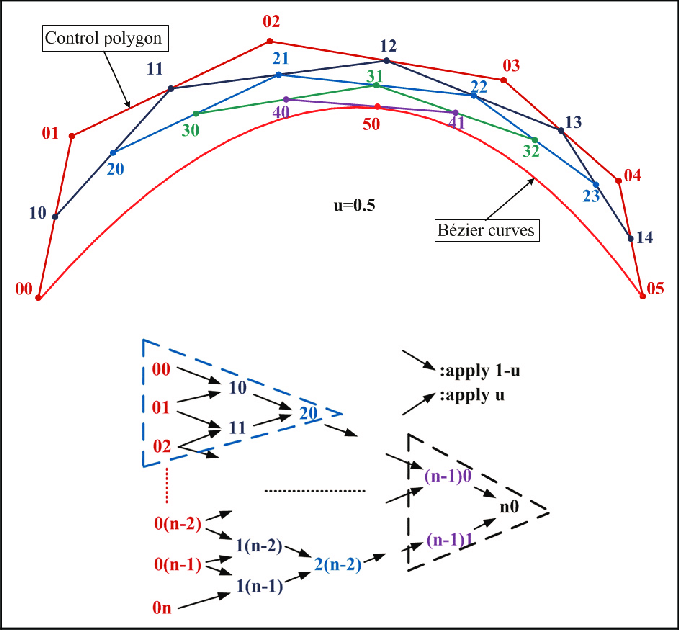
\includegraphics[height=9cm]{figures/General-process-of-De-Casteljau-algorithm.png}
    \caption{De-Casteljau Algorithm, from \cite{Wang-spline}}  
    \label{fig:De-casteljau-algo}
\end{figure}

\subsection{Derivative of Bezier curve}
\label{subsec:Derivative of Bezier curve}
\subsubsection{1st Method}
We use : 
\[
    p^{(k)} = \frac{ n!  }{ \left( n-k\right) ! } \sum_{k=0}^{n-k} \Delta^k P_i B _{ i }^{
    n-k} (t) 
\]
then we calculate $ \Delta ^k P_i  $ given by the De Casteljau algorithm on $ \Delta^kP_i
$.
When k = 0 
\[
\underbrace{
\begin{pmatrix*}
    P_0  \\
    P_1 \\
    \vdots \\
    P_n 
\end{pmatrix*}
\to  
\begin{pmatrix*}
    \Delta P_0  \\
    \Delta P_1 \\
    \vdots \\
    \Delta P_{n-1}  
\end{pmatrix*}
\to 
\begin{pmatrix*}
    \Delta^2 P_0  \\
    \Delta^2 P_1 \\
    \vdots \\ 
    \Delta^2 P_{n-2}  
\end{pmatrix*}}_{ \text{finite differences}} 
\underbrace{
\to 
P''(t) \frac{ 1 }{ n\left( n-1\right)  } }_{\text{De Casteljau}}
\]

\subsubsection{Second Method}
We do not need to calculate $ \Delta^k P_i  $. 
\begin{prop}[]
   \[
       P^{(k)} (t) = \frac{ n!  }{ \left( n-k\right) ! } \Delta ^k P _{ 0 }^{ \left( n-k\right)  } 
   \] 
    \label{def:}
\end{prop}

Thus, for $ k = 1 $ we have 
\[
    P'(t) = n\left( P _{ 1 }^{ (n-1)  } - P _{ 0 }^{ (n-1) } \right) 
\]
k=2 

\[
    P''(t) = n(n-1)\left( P _{ 1 }^{ (n-2)  } -2P _{ 1 }^{ (n-2) } +  P _{ 0 }^{ (n-2) } \right) 
\]
Intuition of the proof : 
\begin{align*}
    \Delta P_0  &= P_1 - P_0  \\
    \Delta P_1  &= P_2 - P_1  \\
    \text{ Which Gives }& \\
     &= \left( 1-t\right) \left( P_1 - P_0 \right) + t\left( P_2 - P_1 \right)  \\ 
      &= \left( 1-t\right) P_1 + tP_2  \\ 
       &= - \left( \left( 1-t\right) P_0 + P_1\right)  \\ 
\end{align*}


\section{Tutorial 2: Bézier Curves and Bernstein polynomials}
\label{sec:Tutorial 2: Bézier Curves and Bernstein polynomials}
\subsubsection{Exercise 1 (Bernstein polynomials)} 
Show the following : 
\begin{enumerate}
    \item Linear precision : 
        \[
            \sum_{i=0}^{n} \frac{ i }{ n  } B^n_i(t) = t \quad \forall t\in [0,1], \
            \forall n > 0, \ \forall i \in \set{ 0,\dots, n } 
        \]
    \item Recursive formula 
        \[
            B^n_i(t) = \left( 1-t\right) B _{ i }^{ n-1 } (t) + tB _{ i-1 }^{ n-1 } (t)
            \quad \forall n > 0, \ \forall i \in \set{ 0, \dots, n } 
        \]
    \item The family of Bézier polynomials $ \left( B_9\right) _{ 0\leq i \leq n  }^{  }
        $ is a basis of the space of polynomials of degree $ \leq n  $. 
\end{enumerate}
\subsubsection{Exercise 2}
Let $ P_0 $ and $ P_1 $ be two points of $ \mathbb{R}^d $. Descrie the Bézier curve
associated to $ P_0 $ and $ P_1 $. 

\subsubsection{Exercise 3}
Let $ \mathcal{ A }  $ be the affine space identified to $ \mathbb{R}^2 $ and $ \gamma $
be the parameterized curve 
\begin{align*}
    \gamma :  [0,1] &\to \mathbb{R}^2  \\ 
     t &\to \left( t,t^2\right)  \\ 
\end{align*}
\begin{enumerate}
    \item Express $ \gamma $ in the monomial basis. 
    \item Express $ \gamma $ in the Bernstein polyonimals basis. 
    \item Give the control polygon of $ \gamma $. Make a drawing with the curve and
        control polygon. 
\end{enumerate}

\subsubsection{Exercise 4}
Let $ [)_0, \cdots, P_6]  $ be a control polygon and : 
\begin{itemize}
  \item Express the condition on the $ P_i $ to ensure that the Bézier curve 
      \[
          P(t) = \sum_{i=0}^{6} P_iB^6_i(t) 
      \]
      is closed of class $ \mathscr{ C } ^2 $.
  \item Draw an example of such a control polygon.
\end{itemize}

\subsubsection{Exercise 5 (Bézier Function) }
A Bézier function is a curve of the form 
\begin{align*}
    f : [0,1] &\to \mathbb{R}\\
    t &\to \sum_{i=0}^{n} \lambda_i B_i^n(t) 
\end{align*}
Show that the graph  $ G(f) \coloneqq \set{ \left( x,f(x)\right) , x \in [0,1] }  $ of the
function $ f $ is a Bézier curve associated to the points $ P_i = \left( i/n, \lambda_i
\right)  $.

\subsubsection{Exercise 6}
Let $ f(t) = \sum_{i=0}^{n} \lambda_iB^n_i(t)  $ be a Bézier function. 
\begin{enumerate}
    \item Show that 
        \[
        \int\limits_{0}^{1} f(t) \ dt = \frac{ \lambda_0 + \dots + \lambda_n }{ n+1 } 
        \]
        hint : consider the primitive F of f
    \item In particular, show that 
        \[
            \int\limits_{0}^{1} B^n_i(t) = \frac{ 1 }{ n+1 } 
        \]
\end{enumerate}
\subsubsection{Exercise 7 (Degree elevation) }
The idea is to use the observation that a polynomial curve $ P $ of degree $ \leq n  $ can
be seen as a polynomial curve of degree $ \leq n+1 $, namely 
\[
    P(t) = \sum_{i=0}^{n} P_iB^n_i(t) = \sum_{i=0}^{n+1} Q_iB _{ i }^{ n+1 } (t) 
\] 
\begin{enumerate}
    \item Show that 
        \[
            B _{ i }^{ n  } (t) = \frac{ n+1 - i }{ n+1 } B _{ i }^{ n+1 } (t) + \frac{
            n+1  }{ i+1 } (t) 
        \]
    \item Calculate $ Q_i $ in terms of the $ P_j $'s
\end{enumerate}


\subsection{Solutions}
\label{subsec:Solutions}
\subsubsection{1) }
\begin{enumerate}
    \item 
        The first index vanishes, so we can rewrite the sum as 
        \[
            \sum_{i=1}^{n} \frac{ i }{ n  }  B _{ i  }^{ n  } (t) 
        \]
        Furthermore, 
        \[
        i \begin{pmatrix*}
            n   \\
            i  
        \end{pmatrix*}
        = \frac{ n\left( n-1\right) !  }{ \left( i-1\right) !\left( n-i\right) ! } = 
        n\begin{pmatrix*}
            n-1  \\
            i-1  
        \end{pmatrix*}
         
        \]
        Thus, we have, for the first iteration of the sum 
        \[
            \frac{ n   }{ n  } \frac{ \left( n-1\right) ! }{ \left( n-1\right) ! }  
            t\left( 1-t\right) ^{n-1} = t\left( 1-t\right) ^{n-1} = t \left( B _{ 0 }^{
            n-1 } (t) \right) 
        \]
        which allows us to rewrite the sum as 
        \[
            t\sum_{i=0}^{n} B _{ i }^{ n  } (t)  = t\left( 1\right) = t
        \]
    \item 
        \begin{align*}
            B _{ i }^{ n  } (t) &= \left( 1-t\right) B _{ i }^{ n-1 } (t) + tB _{ i-1 }^{
            n-1 } (t) \\
                                &= \left( 1-t\right) \begin{pmatrix*}
                                    n-1  \\
                                     i 
                                \end{pmatrix*}
                                t^i\left( 1-t\right)^{n-1-i} + t 
                                \begin{pmatrix*}
                                    n-1  \\
                                    i-1  
                                \end{pmatrix*}
                                t^{i-1}\left( 1-t\right) ^{n-1 - (i-1)}\\ 
                                 &= \begin{pmatrix*}
                                     n-1  \\
                                     i  
                                 \end{pmatrix*}
                                 t^i\left( 1-t\right) ^{n-i} +
                                 \begin{pmatrix*}
                                     n-1  \\
                                     i-1  
                                 \end{pmatrix*}
                                 t^i\left( 1-t\right) ^{n-i}\\
                                  &= \left( \begin{pmatrix*}
                                      n-1  \\
                                      i  
                                  \end{pmatrix*}
                                  + 
                                  \begin{pmatrix*}
                                      n-1  \\
                                      i-1  
                                  \end{pmatrix*}
                              \right) t^i\left( 1-t\right) ^{n-i}  \\
                               &= \begin{pmatrix*}
                                   n   \\
                                   i  
                               \end{pmatrix*}
                               t^i\left( 1-t\right) ^{n-i} = B _{ i }^{ n  } (t) \\ 
            \end{align*}
        \item To show $ B _{ i }^{ n  } (t) $ as a basis of the space of polynomials of
            degree $ \leq n  $ we use derivation. 
            Consider how 
            \[
                B _{ i }^{ n  } (t) \implies \begin{pmatrix*}
                    n   \\
                    i  
                \end{pmatrix*} t^i
                \left( P \right)  
            \]
            where $ P $ is some polynomial. Then we can write this as a sum under the form 
            \[
            \alpha_0\left( P\right) + \alpha_1t\left( P\right) + \cdots  + \alpha_nt^n = 0
            \]
            We check each $ \alpha_i $. Firstly, taking the derivative of this polynomial
            gives us 
            \[
                \alpha_1\left( P\right) + \cdots  + n\alpha_nt^{n-1} = 0
            \]
            Then $ \alpha_0 = 0 $, this can be done iteratively for each $ \alpha_i $.
            Then $ B _{ i  }^{ n  } (t)  $ is a linear independent set and a basis for
            polynomials of degree $ \leq n $.  
\end{enumerate}

\subsubsection{2)}
The Bézier curve consisting of only 2 points is the straight line :  
\begin{align*}
    P(t) &= \sum_{i=0}^{1} P_iB _{ i }^{ n  } (t) \\
     &= P_0\left( 1-t\right) + P_1t \\ 
      &= P_0 + \left( P_1 - P_0\right) t \\ 
\end{align*}

\subsubsection{3)}
\begin{enumerate}
  \item The monomial basis has representation 
      \[
      \begin{pmatrix*}
          1  \\
          0  
      \end{pmatrix*}
      t + \begin{pmatrix*}
          0  \\
          1  
      \end{pmatrix*}
      t^2
      \]
  \item Bernstein basis is given by : 
      \[
          B _{ 0 }^{ 2 } (t) = \left( 1-t\right)^2; \quad B _{ 1 }^{ 2 } (t) = 2t\left( 1-t\right)
           ; \quad B _{ 2 }^{ 2 } (t) = t^2
      \]
      which results in the following : 
     \[
     \begin{pmatrix*}
         0  \\
         0  
     \end{pmatrix*}
     B _{ 0 }^{ 2 } (t) + 
     \begin{pmatrix*}
         \frac{ 1 }{ 2 }   \\
         0 
     \end{pmatrix*}
     B _{ 1 }^{ 2 } (t) + \begin{pmatrix*}
         1  \\
         1  
     \end{pmatrix*}
     B _{ 2 }^{ 2 } (t)
     \]
 \item The curve is given by :  
\begin{figure}[ht]
    \centering
    \incfig{e4p3}
    \caption{e4p3}
    \label{fig:e4p3}
\end{figure}
\end{enumerate}

\subsubsection{4)}
\begin{itemize}
  \item In order to ensure that the Bézier curve 
      \[
          P(t) = \sum_{i=0}^{6} P_iB _{ i }^{ 6 } (t) 
      \]
      to be closed of class $ \mathscr{ C } ^2 $ we must have 
      \begin{enumerate}
          \item $P(0) = P(1)$ 
          \item $ P'(0) = P'(1) $
          \item $ P''(0) = P''(1) $
      \end{enumerate}
      Thus, 
      \begin{enumerate}
          \item \[ P_0 = P_n \]
          \item 
              \begin{align*}
                  P'(0) = 6\left( P_1 - P_0\right) &= P'(1) = 6\left( P_5 - P_6\right) \\
                  \vv{P_1P_0} &= \vv{P_5P_6} 
              \end{align*}
          \item 
              \begin{align*}
                  P''(0) = 30\left( P_2 - 2P_1 + P_0\right) &= P''(1) = 30\left( P_4 - 2P_5
                  + P_6\right) \\
                   &\text{ since } P_0 = P_6 \\ 
                  P_2 - 2P_1 &= P_4 - 2P_5 \\
                  \vv{P_2P_4} &= 2\vv{P_1P_5} \\ 
              \end{align*}
      \end{enumerate}
        This system of equations results in the figure : 
\begin{figure}[ht]
    \centering
    \incfig{t2e4}
    \caption{Closed of Class $ \mathscr{ C } ^2 $}
    \label{fig:t2e4}
\end{figure}
\end{itemize}

\subsubsection{5)}
This is found through simple computation. We take 
\[
P_i = \begin{pmatrix*}
    \frac{ i }{ n  }   \\
    \lambda_i   
\end{pmatrix*}
\]
Then 
\begin{align*}
    \sum_{i=0}^{n } \begin{pmatrix*}
        i/n   \\
        \lambda_i   
    \end{pmatrix*}
    B _{ i  }^{ n  } (t) &= \begin{pmatrix*}
        \sum_{i=0}^{n } \frac{ i }{ n  } B _{ i  }^{ n  } (t)   \\
        \sum_{i=0}^{n } \lambda_i B _{ i  }^{ n  } (t)   
    \end{pmatrix*} \\ 
     &= \begin{pmatrix*}
         t  \\
         f(t)  
     \end{pmatrix*}
      \\ 
\end{align*}

\subsubsection{6)}
\begin{enumerate}
    \item 
    \begin{align*}
        \int\limits_{0}^{1} f(t) \ dt
    \end{align*}
\item 
\end{enumerate}

\subsubsection{7)}
\begin{enumerate}
    \item 
        \begin{align*}
            &\frac{ n+1-i }{ n+1 } B _{ i }^{ n+1 } (t) + \frac{ i+1 }{ n+1 }B _{ i+1 }^{
        n+1 } (t)  \\ 
            &=  \frac{ n+1-i }{ n+1 } \begin{pmatrix*}
                n+1  \\
                i  
            \end{pmatrix*}
            t^i\left( 1-t\right) ^{n+1-i} + \frac{ i+1 }{ n+1 } \begin{pmatrix*}
                n+1  \\
                i+1  
            \end{pmatrix*}
            t^{i+1}\left( 1-t\right) ^{n+1-(i+1)} \\ 
            &=  
                \frac{ n! }{ i!\left( n-i\right) ! } 
            t^i\left( 1-t\right) ^{n+1-i} + 
            \frac{n! }{ i!\left( n - i\right)!} 
            t^{i+1}\left( 1-t\right) ^{n-i} \\ 
             &= \begin{pmatrix*}
                 n   \\
                 i  
             \end{pmatrix*}
             t^i\left( 1-t\right) ^{n-i} \left( \left( 1-t\right) + t\right)    
             \\
             &= B _{ i  }^{ n  } (t) \\  
               \\ 
        \end{align*} 
    \item We begin by expanding using the form above : 
        \begin{align*}
            \sum_{i=0}^{n } P_iB _{ i }^{ n  } (t) &= \sum_{i=0}^{n }P_i \left( \frac{ n+1-i
            }{ n+1 }B _{ i }^{ n+1 } (t) + \frac{ i+1 }{ n+1 } B _{ i+1 }^{ n+1 }
        (t)\right) \\
                                                   &= \sum_{i=0}^{n} \frac{ n+1-i }{ n+1 }
                                                   P_iB _{ i }^{ n+1 } (t) +
                                                   \sum_{i=1}^{n+1} \frac{ i }{ n+1 } 
                                                   P_{i-1}B _{ i }^{ n+1 }  \\ 
                                                   &= P_0B _{ 0 }^{ n+1 } (t) +
                                                   \sum_{i=1}^{n} \left( P_i \frac{ n+1-i
                                                   }{ n+1 } + P_{i-1} \frac{ i }{ n+1 }
                                               \right) B _{ i }^{ n+1 } (t) + P_nB _{ n+1
                                           }^{ n+1 }  \\ 
        \end{align*} 
\end{enumerate}



\chapter{Curves in the Plane}
\section{Introduction}
\label{sec:Introduction}

To represent them, we use 
\begin{defn}[Parametrized Curves]
    \begin{align*}
        \gamma : [a,b] &\to \mathbb{R}^d \\
        t &\to \gamma(t)  
    \end{align*}
    \label{def:Parametrized Curves}
\end{defn}

\begin{figure}[ht]
    \centering
    \incfig{planar-curve}
    \caption{Parametrized Planar Curve}
    \label{fig:planar-curve}
\end{figure}


\begin{defn}[Implicit Curves]
    Let $ f : \mathbb{R}^2 \to \mathbb{R} $
    then $ f^{-1} ( \set{ 0 } ) = \set{ (x,y) \in \mathbb{R}^2, f(x,y) = 0 }  $
    is a curve.
    \label{def:Implicit Curves}
\end{defn}

\begin{exmp}[]
    \[
        f(x,y) = x^2 + y^2 -1 
    \]
\end{exmp}

\begin{figure}[ht]
    \centering
    \incfig{example313}
    \caption{Example 3.1.3}
    \label{fig:example313}
\end{figure}


\begin{defn}[Graphs of Functions]
    $ \varphi : [a,b] \to \mathbb{R} $. 
    \[
        \text{graph} \left( \varphi\right) = \set{ \left( t, f(t) \right) , t \in [a,b]  } 
    \]
    \label{def:Graphs of Functions}
\end{defn}

\newpage
\begin{exmp}[]
    $ \varphi = \sqrt{1 - t^2}  $ and $ t \in [-1,1]  $ then 
\end{exmp}

\begin{figure}[ht]
    \centering
    \incfig{example315}
    \caption{Example 3.1.5}
    \label{fig:example315}
\end{figure}





\section{Generalities on Paramaterized Curves}
\label{sec:Generalities on Paramaterized Curves}
\subsection{Reminder}
\label{subsec:Reminder}
Let $ f:[a,b] \to \mathbb{R}^2\in \mathscr{ C } ^n $ and $ t_0 \in [a,b] $ then 
\[
    f(t) = f(t_0) + \left( t-t_0\right) f'(t_0) + \frac{ \left( t-t_0\right) ^2 }{ 2!  }
    f''(t_0) + \dots + \frac{ \left( t-t_0\right) ^n }{ n! } f^{(n)} (t_0) + \mathcal{ O
    } \left( \left( t-t_0\right) ^n\right) 
\]

In particular, 
\[
    \frac{ f(t) - f(t_0)  }{ t - t_0  } = f'(t_0) 
\]
let curve be $ \mathscr{ C } = \set{ f(t) }  $ and $ f(t_0) \in \mathscr{ C }  $ and $
f'(t_0)  $ is a vector tangent to $ \mathscr{ C }  $ at $ f(t_0)  $. 

Some notes about 2nd derivative and how it "attracts" the curve. 


\[
    f(t) = f(t_0) + f^{(p)}(t_0) \frac{ \left( t-t_0\right) ^p }{ p! } + \dots + 
    f^{(q)}(t_0) \frac{ \left( t-t_0\right) ^q }{ q! } + \mathcal{ O  } \left( \dots\right) 
\]
p is the smallest k such that $ f^{(k)}(t_0) \neq 0 $ and q is smallest q such that 
\[
    \left( f^{(q)}(t_0),f^{(k)}(t_0)\right)   \text{ independent } 
\]
\newpage
\begin{figure}[ht]
    \centering
    \incfig{linearinependenceoftan}
    \caption{linear independence between derivatives}
    \label{fig:linearinependenceoftan}
\end{figure}

Certain characteristics of the curve can be given by the values of $ p,q $. 


\begin{figure}[ht]
    \centering
    \incfig{pqcurvecharacteristics}
    \caption{pqCurveCharacteristics}
    \label{fig:pqcurvecharacteristics}
\end{figure}

These values then blah blah blah
$ \\ $
\newpage


\section{Parametrization and Geometric Curves}
\label{sec:Parametrization and Geometric Curves}
\begin{defn}[Parametrized Curve]
    A Paramterized curve of class $ \mathscr{ C } ^k $ is a map $ f: I \subset
    \mathbb{R}\to \mathbb{R}^3 \in \mathscr{ C } ^k$, where I is a union of intervals. We
    denote $ \left( I, f\right)  $ such a curve.
    \label{def:Parametrized Curve}
\end{defn }

Remark : 
\[
    F(I) \coloneqq \mathscr{ C } 
\]
is the geometric support. Interval connected $ \implies \mathscr{ C }  $ is connected. 
I compact set $ \implies \mathscr{ C }  $ compact set. 
$ \\ $
Remark : 
$ \\ $
Some curve may have 2 paramterization without the same regularity. 
\begin{exmp}[]
    \begin{align*}
        t &\to \left( t, t^{3/2}\right) t > 0  \\ 
        t &\to \left( \left | t \right | , - \sqrt{t^3}\right) t \leq 0  \\ 
    \end{align*}
    another parametrization is 
    \[
        t \to \left( t^2, t^3\right) \in \mathscr{ C } ^{\infty} 
    \]
\end{exmp}
 

\newpage 
\subsection{ReParametrization}
\label{subsec:ReParametrization}
Let $ f : I \to \mathbb{R}^3 $ param curve in $ \mathscr{ C } ^k $ and $ e : J \to I $ is
a $ \mathscr{ C } ^k $ diffeomorphism (bijective, $ e'(x) \neq 0, \mathscr{ C } ^k $. 
Then $ f \circ e : J \to \mathbb{R}^3 $ has the same "geometric curve" and we say that 
\begin{itemize}
  \item $ f\circ e $ is a reparametrization of $ f $
  \item $ e $ is called an admissible change of variable
\end{itemize}


\begin{figure}[ht]
    \centering
    \incfig{reparamaterized-curve}
    \caption{Reparamaterized Curve}
    \label{fig:reparamaterized-curve}
\end{figure}


We consider the following equivalence class 
\begin{defn}[Equivalence Class for Curves]
    $ \\ $
    $ \left( I,f\right) \sim \left( J,g\right)  $ if 
    $
    \exists e : J \to I,  g = f \circ e  \text{ e admissible change of variable} 
    $
    \label{def:}
\end{defn}

\begin{defn}[Geometric Curve]
    A geometric curve is an equivalence class of this relation
    \label{def:Geometric Curve}
\end{defn}

\section{Regular Curve}
\label{sec:Regular Curve}

\begin{defn}[Regular Curve]
    Let $ k \geq 1 $. 
    We say that a paramatrized curve $ \left( f,I\right)  $ of class $ \mathscr{ C } ^k $
    is regular if 
    \[
        f'(t) \neq 0 \ \forall t \in I
    \]
    A geometric curve is regular if there exists a paramatrized which is regular. 
    \label{def:Regular Curve}
\end{defn}

If $ \mathscr{ C } $ is of class $ \mathscr{ C } ^1 $, then there exists $ f: I \to
\mathscr{ C }  $, where $ \mathscr{ C } = f\left( I\right)  $ 
\[
    f'(t) \neq 0 \quad f'(t) \text{ is tangent to } \mathscr{ C } ^k \text{ at } f(t)
\]

If $ \left( I,f\right)  $ is regular then every reparametrization $ \left( J,g \right)  $ 
is also regular. Indeed : $ \forall t, \ f'(t) \neq 0  $ gives 
\[
    g = f \circ e \implies \forall t,  \ g'(t) = \underbrace{f'(e(t))}_{\neq 0} \times 
    \underbrace{e'(t)}_{\neq 0}  \neq 0
\]

\begin{exmp}[]
    A line segment in $ \mathbb{R}^2 $ with $ t \to \left( t, at+b\right)  $ regular,
    can also be
    reparametrizated by $ t\to \left( t^3, at^3+b\right)  $ non regular. The reason for this is 
    \[
        f'(t) = \left( 3t^2, 3at^2\right) = 0 \text{ at } x = 0
    \]
\end{exmp}
\subsubsection{Remark}
This curve does not admit a regular paramatrization. 

    
\begin{figure}[ht]
    \centering
    \incfig{regular-and-non-regular-curves}
    \caption{Regular and Non-regular curves}
    \label{fig:regular-and-non-regular-curves}
\end{figure}

However, this is not to say that there does not exist parametrizations of these figures,
it is just to say that $ f'(a) = 0 $ where a is the non-smooth point. 

Furthermore, we have 


\begin{figure}[ht]
    \centering
    \incfig{c1-but-not-c2}
    \caption{ $ \mathscr{ C } ^1 $ but not $ \mathscr{ C } ^2 $}
    \label{fig:c1-but-not-c2}
\end{figure}

This curve is $ \mathscr{ C } ^1 $ since $ f''(x) = 0 $. 
\newpage 

\section{Metric Properties of Curves}
\label{sec:Metric Properties of Curves}
\subsection{Length of curves}
\label{subsec:Length of curves}
\begin{defn}[Length of a curve]
    Let $ f : I = [a,b] \to \mathbb{R}^d $. We see that the straight line segments 
    obviously have less length than $ \mathscr{ C }  $. $ \\ $
    Let $ \mathscr{ S }  = \set{ \text{ subdivisions } a=t_0 < \dots < t_n = b } $.

    For $ s \in \mathscr{ S }   $ we denote 
    \[
        \gamma(s) = \sum_{i=0}^{N-1} \| f(t_{i+1}) - f(t_i) \|^{ }_{ }  
    \]If $ \set{ \gamma(s), s \in \mathscr{ S }   }  $ is bounded we say that $ f $ is
    rectifiable. Its lengh is defined by 
    \[
        \gamma(f) = \sup_{s \in \mathscr{ S } } \gamma(s)
    \]
    Then If $ f:[a,b] \to \mathbb{R}^d $ is $ \mathscr{ C } ^1 $ then $ f $ is rectifiable
    and 
    \[
        \gamma(f) = \int\limits_{a}^{b} \| f'(t) \|^{ }_{ } \ dt
    \]
    \label{def:Length of a curve}
\end{defn}
Sketch of proof $ \\ $

\begin{align*}
    \int\limits_{a}^{b} \| f'(t)  \|^{ }_{ } \ dt &= \sum_{i=1}^{n-1}
    \int\limits_{t_i}^{t_{i+1}} \| f'(t)  \|^{ }_{ } \ dt \\ 
\end{align*}
The right hand side of this term gives us 
\begin{align*}
     &\sim \left( t_{i+1} - t_i \right) \| f'(t) \|^{ }_{ }   \\ 
     &\sim \left( t_{i+1} - t_i \right) \frac{ \| f(t_{i+1} - f(t_i)  )  \|^{ }_{ }  }{
     \left | t_{i+1} - t_i \right |  }   \\ 
\end{align*}

\begin{figure}[ht]
    \centering
    \incfig{length-of-a-curve}
    \caption{Length of a Curve}
    \label{fig:length-of-a-curve}
\end{figure}





\subsection{Arc Length Parametrization}
\label{subsec:Arc Length Parametrization}
\begin{defn}[]
    Let $ \left( I,f\right) \in \mathscr{ C } ^1 $ where $ I = [a,b] ,\ t_0 \in I $. We
    call arc-length the map 
    \begin{align*}
        \simga: I &\to \mathbb{R}  \\
        t &\to \int\limits_{t_0}^{t} \| f'(\mu) \|^{ }_{ } \ d\mu \\ 
    \end{align*} 
    \label{def:}
\end{defn}
\subsubsection{Remark}
$ \left | \sigma(t) \right |  $ is the length of the curve between $ f(t)  $ and $ f(t_0)
$ where $ \sigma(t) < 0 \iff t<t_0 $
\subsubsection{Remark}
If $ f $ is regular then $ \sigma  $ is strictly increasing and $ \sigma'(t) = \| f'(t)
\|^{ }_{ } > 0 $, therefore, $ \sigma  $ is an admissable change of variable of class $
\mathscr{ C } ^1 $

\begin{defn}[]
    $ f\circ \sigma^{-1} $ is an arc-length paramatrization of the curve. 
    \label{def:}
\end{defn}
So every $ \mathscr{ C } ^1 $ regular curve admits an arc-length paramatrization.
We use, by convention, $ S $ as the parameter of the arc-length parametrization.

\begin{figure}[ht]
    \centering
    \incfig{arc-length-paramatrization}
    \caption{Arc-length Paramatrization}
    \label{fig:arc-length-paramatrization}
\end{figure}








\begin{prop}[]
    \begin{itemize}
      \item  The arc-length paramatrization is unique up to the parameter $ t_0 $ if $ I = [a,b],\
    t_0 = a $.
\item $ \forall s \in J, \ \| f'(s) \|^{ }_{ } = 1 $ if $ f $ arc-length param 
\item $ \forall s \in J, f'(s) \perp f''(s)  $ for $ f $ arc-length
    \end{itemize}  
\end{prop}
\begin{proof}
    Let $ g $ be any parametrization and $ f = g \circ \sigma^{-1}  $. Then 
    \[
        \forall s \ f'(s) = g'\left( \sigma^{-1} (s) \right) \times \left(
        \sigma^{-1}\right) '(s) = \frac{ g'\left( \sigma^{-1}(s)\right)  }{ \| g'\left(
    \sigma^{-1}(s)\right)  \|^{ }_{ }  } 
    \]
    where 
    \[ \left( \sigma^{-1}\right)' (s) = \frac{ 1 }{ \sigma'\left(\sigma^{-1}(s)\right) } = 
    \frac{ 1 }{ \| g'\left( \sigma^{-1}(s)\right)  \|^{ }_{ }  } \]
    Then $ \| f'(s) \|^{ }_{ } = 1 $ and 
    \[
        \forall s \in J \ \| f'(s) \|^{ 2}_{ } = \langle f'(s) , f'(s) \rangle = 1
    \]
    We derive, $ \forall s \in J  $
    \[
        2 \langle f''(s)  , f'(s)  \rangle = 0 \implies f''(s) \perp f'(s)
    \]
\end{proof}

\section{Planar Curves}
\label{sec:Planar Curves}
\subsection{Serret-Fresnet Frame}
\label{subsec:Serret-Fresnet Frame}
Let $ f : I \to \mathbb{R}^2, \in \mathscr{ C } ^1 $-regular. Then 
\[
    T(t) = \frac{ f'(t)  }{ \| f'(t) \|^{ }_{ }  } \quad N(t) = \text{rot}_{ \frac{ \pi }{
    2}} \left( T(t)\right) 
\]
So $ \left( f(t), \boldsymbol{T}(t), \boldsymbol{N} (t) \right)  $ is a frame that is
called the Serret-Fresnet Frame.

\subsubsection{Remark}
If arc-length then we have 
\[
    T(s) = f'(s) \qquad N(s) = \text{rot} _{ \frac{ \pi }{ 2 } }\left( T(s)\right) 
\]

\subsection{Curvature}
\label{subsec:Curvature}
\begin{defn}[Curvature]
    Let $ f : I \to \mathbb{R}^2 $ arc-length. The curvature at $ f(s)  $ is defined by 
    \[
        k(s) \coloneqq \langle f''(s)  , N(s)  \rangle = \pm \| f''(s) \|^{ }_{ } 
    \]
    \label{def:Curvature}
\end{defn}
\begin{prop}[]
    Let $ f : I \to \mathbb{R} $ any parametrization. Then 
    \[
        k(u) = \frac{ \text{det} \left( f'(u), f''(u) \right)  }{ \| f'(u) \|^{3 }_{ }  } 
    \]
    \label{def:}
\end{prop}

\begin{proof}
    We denote $ \overline{f} = f \circ \sigma^{-1}  $ the arc-length parametrization. We
    put $ u = \sigma^{-1}(s)  $. Then 
    \begin{align*}
        \overline{f}'(s) &= f'\left( \sigma^{-1}(s) \right) \frac{ 1 }{ \| f'\left( \sigma^{-1}
        (s)\right)  \|^{ }_{ }  }  \\
                     &= \frac{ f'(u) }{ \| f'(u) \|^{ }_{ }  }  \\ 
    \end{align*}
    We derive again 
    \begin{align*}
        \overline{f}''(s)  &= \frac{ f''(u) }{ \| f'(u) \|^{2 }_{ }  } + f'(u) \frac{ d }{
        ds}  \\ 
    \end{align*}
    where $ \frac{ d }{ ds }  $ is the real value result of the rhs above 
    \begin{align*}
        \text{det} \left( \overline{f}'(s), \overline{f}''(s) \right)  &= \text{det}
        \left( \frac{ f'(u) }{ \| f'(u) \|^{ }_{ }} , \frac{ f''(u) }{ \| f'(u) \|^{2 }_{
            }}
        + \lambda u f'(u)   \right)  \\ 
                                                                       &=
                                                                       \frac{\text{det}
                                                                       \left(f'(u), f''(u)
                                                                   \right)  }{ \| f'(u)
                                                               \|^{3 }_{ }   }  \\ 
    \end{align*}
    And 
    \begin{align*}
        \text{det} \left( \overline{f}'(s) , \overline{f}''(s) \right) &= \text{det} \left( T(s),
        k(s)N(s)\right) \\
        &= k(s)
    \end{align*}
    since, 
    \[
        f''(s) = k(s)N(s) 
    \]
    \[
        k(s) \coloneqq \langle f''(s) , N(s) \rangle = \pm \| f''(s) \|^{ }_{ } 
    \]
\end{proof}

\begin{figure}[ht]
    \centering
    \incfig{curvature}
    \caption{curvature}
    \label{fig:curvature}
\end{figure}








\subsection{Osculating Circle and Center of Curvature}
\label{subsec:Osculating Circle and Center of Curvature}
\begin{defn}[]
    \[
        c(t) = f(t) + \frac{ 1 }{ k(t) } N(t) 
    \]
    is called the center of curvature. 
    \[
        \frac{ 1 }{ \left | k(t) \right |  } 
    \]
    is the radius of curvature at $ f(t) $
    The circle 
    \[
        \mathscr{ C } \left( c(t), \frac{ 1 }{ \left | k(t) \right |  } \right) 
    \]
    The evolute of $ f $ is the set of centers of curvatures.
\end{defn}


\subsection{Serret-Fresnet Formula}
\label{subsec:Serret-Fresnet Formula}
\begin{prop}[]
    \[
        T'(s) = k(s)N(s) \qquad N'(s) = -k(s)T(s)  
    \]
    lhs done is done, and rhs is by definition 
\end{prop}

\subsection{Total Curvature}
\label{subsec:Total Curvature}

\begin{ftheo}[Total Curvature]
    Let $ f: I \subset \mathbb{R}\to \mathbb{R}^2 $ planar curve parametrized by
    arc-length, then 
    \[
        \int\limits_{a}^{b} k(s) \ ds = \theta(a,b)
    \]
    is the angle between the two tangents at a and b.
    \label{th:Total Curvature}
\end{ftheo}


\begin{proof}
    \[
        f(s) = \begin{pmatrix*}
            x(s)  \\
            y(s)  
        \end{pmatrix*}
        \quad \theta (s) = \left( (o,x) , T(s) \right) 
    \]
    where $ o  $ is the angle between tangent and the x? 
    Then 
    \[
        T(s) = \begin{pmatrix*}
            \cos \theta (s)   \\
            \sin \theta (s)   \\
        \end{pmatrix*}
        \quad 
        N(s) = 
        \begin{pmatrix*}
            -\sin \theta (s)  \\
            \cos \theta (s)   
        \end{pmatrix*}
        
    \]
    However, 
    \[
        T'(s) = k(s) N(s) \quad \text{ and } T'(s) = \theta '(s) N(s) 
    \]
    then 
    $ \theta '(s) = k(s)  $. 
    then 
    \[
        \int\limits_{a}^{b} \theta '(s) ds = \theta(b) - \theta(a) 
    \]
    which is the difference between the angles. 
\end{proof}

\begin{figure}[ht]
    \centering
    \incfig{total-curvature}
    \caption{Total Curvature}
    \label{fig:total-curvature}
\end{figure}

In figure \ref{fig:total-curvature} we have $ \theta_1\left( a,b\right) = \theta_2\left(
a,b\right) = \theta_3\left( a,b\right) + 6\pi $. We defined the "winding number" as an
index refering to the full revolutions around the a curve that is closed of class $
\mathscr{ C } ^2 $.  

\[
    k = \frac{ l }{ 2\pi  } \int\limits_{a}^{b} k(s) \ ds \in \mathbb{Z}
\]


\begin{figure}[ht]
    \centering
    \incfig{winding-numbers}
    \caption{Winding Numbers}
    \label{fig:winding-numbers}
\end{figure}

\subsubsection{Concluding Thoughts}
\begin{itemize}
  \item Metrics of a curve are given by the 1st derivative
  \item Them shape of a curve is given by the second derivative. 
  \item Arc length parametrization gives constant speed along the curve 
\end{itemize}







\chapter{The Time Variable}
\section{Class notes} 

\includepdf[pages={29-34}]{sources/polyEDP-M1-main.pdf}

\printbibliography

\end{document}
